%% ============================================================
%%  AMS517 — Optimal Trade Execution via Risk-Averse RL
%%  Beamer  |  aspectratio=169  |  ~30 min
%% ============================================================
\documentclass[aspectratio=169, 10pt]{beamer}

\usetheme{Madrid}
\usefonttheme{serif}

%% Colour palette — keep Madrid structure, fix visible colours
\definecolor{myblue}{RGB}{37,99,235}
\definecolor{myred}{RGB}{220,38,38}
\definecolor{mygreen}{RGB}{22,163,74}
\definecolor{myorange}{RGB}{217,119,6}
\definecolor{mypurple}{RGB}{109,40,217}

\setbeamercolor{palette primary}   {bg=myblue,  fg=white}
\setbeamercolor{palette secondary} {bg=myblue!80,fg=white}
\setbeamercolor{palette tertiary}  {bg=myblue!60,fg=white}
\setbeamercolor{palette quaternary}{bg=myblue,  fg=white}
\setbeamercolor{structure}{fg=myblue}
\setbeamercolor{frametitle}{bg=myblue, fg=white}

%% --- ИСПРАВЛЕНИЕ БЛОКОВ ---
%% Отключаем тени, из-за которых появляется черный цвет
\setbeamertemplate{blocks}[rounded][shadow=false]

%% Обычные блоки (синие)
\setbeamercolor{block title}{bg=myblue, fg=white}
\setbeamercolor{block body} {bg=myblue!10, fg=black}

%% Выделенные блоки (красные - alertblock)
\setbeamercolor{block title alerted}{bg=myred, fg=white}
\setbeamercolor{block body alerted} {bg=myred!10, fg=black}

%% Цвет выделенного текста
\setbeamercolor{alerted text}{fg=myred}

\usepackage{amsmath,amssymb, bm}
\usepackage{booktabs}
\usepackage{graphicx}
\usepackage{xcolor}
\usepackage{tikz}
\usetikzlibrary{positioning,arrows.meta}
\usepackage{pgfplots}
\pgfplotsset{compat=1.18}
\usepackage{microtype}
\usepackage{qrcode}

\title[Risk-Averse RL for Trade Execution]{%
  Optimal Trade Execution\\[4pt]
  via Risk-Averse Reinforcement Learning}
\subtitle{AMS517 Course Project}
\author{Matvei Lukianov, John Walsh}
\institute{Stony Brook University}
\date{\today}

%% ============================================================
\begin{document}

% ---- TITLE -------------------------------------------------
\begin{frame}
  \titlepage
\end{frame}

% ---- OUTLINE -----------------------------------------------
\begin{frame}{Outline}
  \tableofcontents
\end{frame}

%% ============================================================
\section{Motivation}
%% ============================================================

\begin{frame}{Motivation}
  \begin{itemize}
    \item Execution = market impact + risk
    \item VWAP dominates institutional benchmarks
    \item RL models ignore benchmark constraints
  \end{itemize}
\end{frame}

\begin{frame}{VWAP Benchmark \& Execution Schedule}
  \begin{block}{VWAP Definition}
    $$\text{VWAP} = \frac{\sum_{t} P_t \Delta V_t}{V_T}$$
  \end{block}
  
  \begin{block}{VWAP Execution Schedule}
    $$q_t = X_0 \frac{\Delta V_t}{V_T}$$
    \begin{itemize}
      \item $q_t$: shares traded
      \item $X_0$: initial inventory
      \item $\Delta V_t$: market volume
    \end{itemize}
  \end{block}

  \begin{itemize}
    \item Aligns execution with liquidity
    \item Acts as a benchmark and a constraint, not an optimal policy
  \end{itemize}
\end{frame}

\begin{frame}{The Optimal Execution Problem}
  \begin{columns}[T]
    \begin{column}{0.50\textwidth}
      \textbf{Setting:} Sell $Q$ shares over $[0,T]$
      minimising execution cost.

      \medskip
      \textbf{Core tension:}
      \begin{itemize}
        \item \alert{Execute fast} $\Rightarrow$ large market impact
        \item \alert{Execute slowly} $\Rightarrow$ price risk
      \end{itemize}

      \medskip
      \textbf{Why not TWAP / VWAP?}
      \begin{itemize}
        \item Deterministic — cannot adapt to realised LOB
        \item Low mean cost but \alert{huge tail risk}
        \item Our result: RL beats VWAP in \textbf{81\%} of episodes
      \end{itemize}

      \medskip
      \textbf{Research Question: Can we unify?}
      \begin{itemize}
        \item Optimal execution, RL, Risk measures, and VWAP benchmarking.
        \item Can a \emph{risk-averse} RL agent reduce \textbf{tail} execution costs vs a \emph{risk-neutral} RL agent?
      \end{itemize}
    \end{column}
    
    \begin{column}{0.46\textwidth}
      \centering
      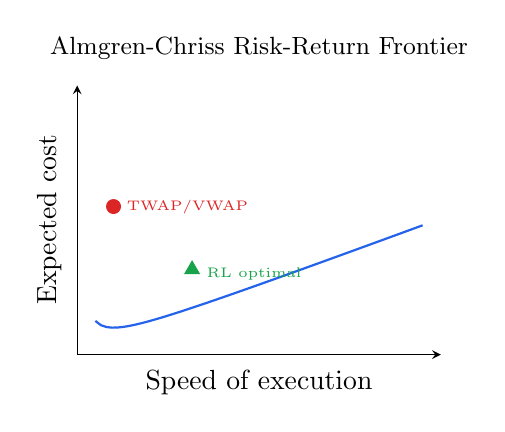
\begin{tikzpicture}
        \begin{axis}[
          xlabel={Speed of execution},
          ylabel={Expected cost},
          xmin=0,xmax=10,ymin=0,ymax=10,
          xtick=\empty,ytick=\empty,
          axis lines=left,width=6.2cm,height=5cm,
          title={\small Almgren-Chriss Risk-Return Frontier}]
          \addplot[myblue,thick,domain=0.5:9.5,samples=60]{0.5/x+0.5*x};
          \addplot[only marks,mark=*,myred,mark size=2.5pt]
            coordinates{(1,5.5)};
          \node[myred,font=\tiny,right] at (axis cs:1.1,5.5){TWAP/VWAP};
          \addplot[only marks,mark=triangle*,mygreen,mark size=3pt]
            coordinates{(3.16,3.16)};
          \node[mygreen,font=\tiny,right] at (axis cs:3.3,3.0){RL optimal};
        \end{axis}
      \end{tikzpicture}
    \end{column}
  \end{columns}
\end{frame}

%% ============================================================
\section{Literature Review}
%% ============================================================

\begin{frame}{Literature Evolution: Three Pillars of the Literature}
  \begin{columns}[T]
    \begin{column}{0.32\textwidth}
      \begin{block}{Almgren \& Chriss (1998)}
        \begin{itemize}\small
          \item Mean-variance optimal liquidation
          \item Linear permanent + temporary impact
          \item Closed-form efficient frontier
          \item \emph{Cannot adapt to market}
        \end{itemize}
        \smallskip
        \footnotesize\textit{We use:} impact model
      \end{block}
    \end{column}
    \begin{column}{0.32\textwidth}
      \begin{block}{Nevmyvaka et al.\ (2006)}
        \begin{itemize}\small
          \item RL on real LOB data (NASDAQ)
          \item State: inv.\ + spread + time
          \item Function approximation
          \item Beats VWAP on 1.5yr data
        \end{itemize}
        \smallskip
        \footnotesize\textit{We use:} LOB state, L1/L2 sweep
      \end{block}
    \end{column}
    \begin{column}{0.32\textwidth}
      \begin{block}{Shen et al.\ (2014)}
        \begin{itemize}\small
          \item Risk Sensitive RL:  Risk-averse RL for trading
          \item TD-error utility: $u(x){=}\text{sgn}(x)|x|^\lambda$
          \item $\lambda{=}0.6$ optimal (Fig.\ 2)
          \item $T{=}10$ decision points
        \end{itemize}
        \smallskip
        \footnotesize\textit{We use:} RA update, $\lambda$, state design
      \end{block}
    \end{column}
  \end{columns}

  \bigskip
  \centering
  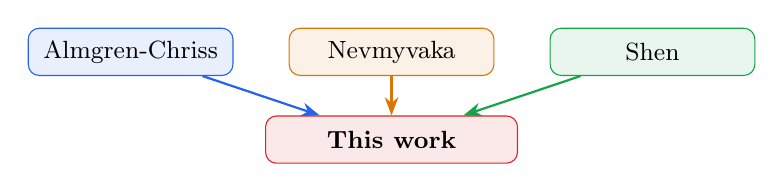
\begin{tikzpicture}[node distance=0.9cm,font=\small]
    \node[draw=myblue,fill=myblue!10,rounded corners,
          minimum width=2.6cm,minimum height=0.6cm](ac){Almgren-Chriss};
    \node[draw=myorange,fill=myorange!10,rounded corners,
          minimum width=2.6cm,minimum height=0.6cm,right=0.7cm of ac](nev){Nevmyvaka};
    \node[draw=mygreen,fill=mygreen!10,rounded corners,
          minimum width=2.6cm,minimum height=0.6cm,right=0.7cm of nev](sh){Shen};
    \node[draw=myred,fill=myred!10,rounded corners,
          minimum width=3.2cm,minimum height=0.6cm,below=0.5cm of nev](us){\textbf{This work}};
    \draw[-{Stealth},myblue,thick](ac)--(us);
    \draw[-{Stealth},myorange,thick](nev)--(us);
    \draw[-{Stealth},mygreen,thick](sh)--(us);
  \end{tikzpicture}
\end{frame}

%% ============================================================
\section{MDP Formulation}
%% ============================================================

\begin{frame}{MDP Formulation}
  \begin{itemize}
    \item \textbf{State:} $S_t = (X_t, t, P_t, V_t, \text{imbalance}, \text{depth})$
    \item \textbf{Action:} $a_t \in [0, X_t]$
    \item \textbf{Inventory Dynamics:} $X_{t+1} = X_t - a_t$ (Simple conservation of shares)
    \item \textbf{Price Impact Model:} $P_{t+1} = P_t - \eta a_t + \epsilon_t$
    \begin{itemize}
      \item $\eta$: market impact coefficient
      \item $\epsilon_t$: noise
    \end{itemize}
    \item \textbf{Reward Function:} $r_t = -C_t - \lambda_1 (a_t - a_t^{VWAP})^2 - \lambda_2 \psi_t$
    \begin{itemize}
      \item Cost + VWAP deviation + risk penalty
    \end{itemize}
  \end{itemize}
\end{frame}

\begin{frame}{Optiver MDP Implementation Details}
  \begin{columns}[T]
    \begin{column}{0.47\textwidth}
      \textbf{State} — 5 continuous features:
      \begin{enumerate}\small
        \item $q_t/Q$ — inventory fraction
        \item $(s_t-\mu_s)/\sigma_s$ — normalised spread
        \item $t/T$ — time fraction
        \item $\text{bid\_sz}_1/(\text{bid\_sz}_1{+}\text{ask\_sz}_1)$ — imbalance
        \item $\text{bid\_sz}_2/\text{bid\_sz}_1$ — book depth
      \end{enumerate}

      \medskip
      \textbf{Actions:} $\{0\%,10\%,\ldots,100\%\}$ of remaining inventory

      \medskip
      \textbf{Reward} (basis points):
      $$r_t = \frac{\bar{p}_t^{\text{exec}} - p_t^{\text{mid}}}{p_0^{\text{mid}}} \times 10^4$$

      \textbf{Terminal:} unexecuted shares dumped
      at 1.5\% discount — forces completion.
    \end{column}
    \begin{column}{0.50\textwidth}
      \textbf{Market impact:}

      \smallskip
      \textbf{Temporary} (Nevmyvaka LOB sweep):
      \begin{enumerate}\small
        \item Execute at \texttt{bid\_price1} up to \texttt{bid\_size1}
        \item Spill to level 2 if $q>\text{bid\_size1}$
        \item Deep-book penalty beyond L1+L2
      \end{enumerate}

      \medskip
      \textbf{Permanent} (Almgren-Chriss Eq.\ 8):
      $$\Delta p^{\text{perm}}_t = \gamma q_t,\quad \gamma = 2\!\times\!10^{-5}$$

      \medskip
      \textbf{Episode:} 10-min Optiver window
      subsampled to $T{=}10$ steps (Shen Sec.\ III-B).
      
      \begin{alertblock}{Inventory calibration}
        \small $Q{=}200\approx$ median L1+L2 depth in Optiver.\\
        $Q{=}2000$: always deep-book $\to$ no learning signal.
      \end{alertblock}
    \end{column}
  \end{columns}
\end{frame}

\begin{frame}{Bellman Equations}
  \begin{block}{Standard Bellman Equation}
    $$V(s) = \max_a \left\{ r(s,a) + \gamma \mathbb{E}[V(s')] \right\}$$
    Core dynamic programming recursion.
  \end{block}

  \begin{block}{Risk-Sensitive Bellman}
    $$V(s) = \max_a \left\{ r(s,a) + \gamma \rho(V(s')) \right\}$$
    $\rho(\cdot)$ = risk functional.
  \end{block}

  \begin{block}{Sample Path Perspective}
    \begin{itemize}
      \item Decisions depend on realized trajectories.
      \item RL approximates sample-path optimization.
    \end{itemize}
  \end{block}
\end{frame}

%% ============================================================
\section{Risk-Averse DQN}
%% ============================================================

\begin{frame}{Risk-Averse DQN: Shen (2014) Update Rule}
  \begin{columns}[T]
    \begin{column}{0.5\textwidth}
      \textbf{Standard (risk-neutral) loss:}
      $$\mathcal{L}_{\text{RN}} = \mathbb{E}[\,\delta_t^2\,]$$

      \textbf{Shen risk-averse loss:}
      $$\mathcal{L}_{\text{RA}} = \mathbb{E}[\,u(\delta_t)^2\,],\quad u(x) = \operatorname{sgn}(x)|x|^\lambda$$

      \textbf{Why $\lambda{=}0.6<1$ is risk-averse:}
      \begin{itemize}
        \item $u(\delta)^2 = |\delta|^{2\lambda}$ — sub-quadratic,\\
              sign cancels: \alert{symmetric} compression
        \item Large $|\delta|$ dampened; small $|\delta|$ amplified
        \item Q-values not inflated by outlier episodes\\
              $\Rightarrow$ \emph{conservative, pessimistic} estimates
      \end{itemize}

      \begin{alertblock}{CVaR is evaluation only}
        \small The utility acts on TD-errors, not returns.\\
        CVaR$_{95}$ is our \textbf{metric}, not the objective.\\
        Distributional RL (QR-DQN) is the next step.
      \end{alertblock}
    \end{column}
    \begin{column}{0.46\textwidth}
      \centering
      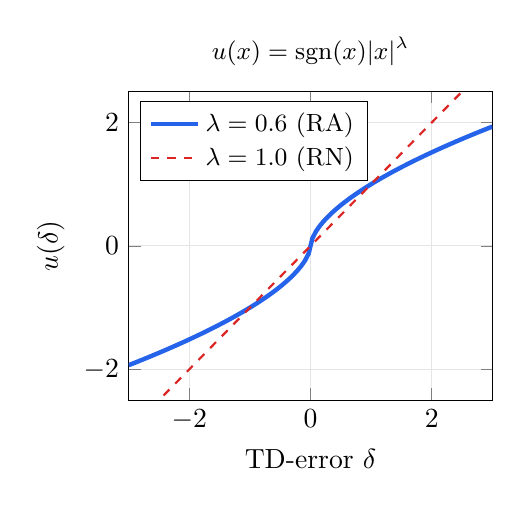
\begin{tikzpicture}
        \begin{axis}[
          width=6.2cm,height=5.5cm,
          xlabel={TD-error $\delta$},ylabel={$u(\delta)$},
          domain=-3:3,samples=100,
          xmin=-3,xmax=3,ymin=-2.5,ymax=2.5,
          legend pos=north west,legend style={font=\small},
          title={\small $u(x)=\operatorname{sgn}(x)|x|^\lambda$},
          grid=major,grid style={gray!20}]
          \addplot[myblue,ultra thick]{sign(x)*abs(x)^0.6};
          \addlegendentry{$\lambda=0.6$ (RA)}
          \addplot[myred,dashed,thick]{x};
          \addlegendentry{$\lambda=1.0$ (RN)}
        \end{axis}
      \end{tikzpicture}

      \smallskip
      \footnotesize
      $u(\delta)^2 = |\delta|^{2\lambda}$: sub-quadratic loss compresses large errors symmetrically $\Rightarrow$ conservative Q-values, not downside asymmetry
    \end{column}
  \end{columns}
\end{frame}

%% ============================================================
\section{Extensions Beyond Shen (2014)}
%% ============================================================

\begin{frame}{Extensions Beyond Shen (2014)}
  \begin{columns}[T]
    \begin{column}{0.48\textwidth}
      \textbf{1.\ Deep Q-Network instead of tabular RL}

      \smallskip
      \begin{tabular}{lll}
        \toprule
        & Shen (2014) & This work \\
        \midrule
        Agent   & Tabular Q    & GPU DQN \\
        Unseen states & Q$=0$ (random) & Interpolated \\
        Stocks  & 1            & \textbf{112} \\
        Episodes & $\sim$1k   & \textbf{386k} \\
        \bottomrule
      \end{tabular}

      \smallskip
      \footnotesize
      Tabular Q cannot generalise — unseen (inv, spread, time)\\
      tuples get zero Q-values $\to$ random policy.\\
      DQN shares weights across similar states.
    \end{column}
    \begin{column}{0.48\textwidth}
      \textbf{2.\ Continuous state instead of one-hot (23 dim)}

      \smallskip
      \begin{tabular}{lll}
        \toprule
        & Shen (2014) & This work \\
        \midrule
        State   & 23-d one-hot & \textbf{5 continuous} \\
        Inventory & 10 buckets & fraction $q/Q$ \\
        Spread  & 3 buckets   & z-score \\
        Extra   & —           & imbalance, depth \\
        \bottomrule
      \end{tabular}

      \smallskip
      \footnotesize
      Network interpolates between states — no bucket boundary artifacts.\\
      LOB imbalance predicts short-term price direction.
    \end{column}
  \end{columns}

  \bigskip
  \begin{block}{What we kept from Shen (2014)}
    \small
    $u(x){=}\operatorname{sgn}(x)|x|^{0.6}$ on TD-error \quad$|$\quad
    $T{=}10$ steps \quad$|$\quad
    Reward in bps \quad$|$\quad
    Inventory $+$ spread $+$ time as core state variables
  \end{block}
\end{frame}

%% ============================================================
\section{Implementation}
%% ============================================================

\begin{frame}{Dataset: Optiver Realized Volatility Prediction}
  \begin{columns}[T]
    \begin{column}{0.5\textwidth}
      \begin{block}{Kaggle Competition (2021)}
        \begin{center}
          \qrcode[height=2cm]{https://kaggle.com/c/optiver-realized-volatility-prediction}

          \vspace{0.3cm}
          \scriptsize Scan for Kaggle dataset
        \end{center}
      \end{block}

      \medskip
      \textbf{Structure:}
      \begin{itemize}\small
        \item \textbf{112 NASDAQ stocks} (anonymized stock IDs)
        \item Each \textbf{time\_id} = one 10-minute auction window
        \item Snapshots every few seconds (up to 600 rows per window)
        \item Fields: \texttt{seconds\_in\_bucket}, bid/ask price \& size, levels 1 \& 2
      \end{itemize}
    \end{column}
    \begin{column}{0.44\textwidth}
      \textbf{LOB snapshot format:}

      \medskip
      \renewcommand{\arraystretch}{1.2}
      \begin{tabular}{ll}
        \toprule
        Column & Description \\
        \midrule
        \texttt{bid\_price1} & Best bid \\
        \texttt{bid\_size1}  & Qty at best bid \\
        \texttt{bid\_price2} & 2nd bid level \\
        \texttt{bid\_size2}  & Qty at level 2 \\
        \texttt{ask\_price1} & Best ask \\
        \texttt{ask\_size1}  & Qty at best ask \\
        \bottomrule
      \end{tabular}

      \medskip
      \textbf{Scale:}
      \begin{itemize}\small
        \item Train: 428,932 total episodes
        \item 90/10 split $\to$ 386k train / 42.9k test
        \item Median \texttt{bid\_size1} $\approx 100$ shares\\
          $\Rightarrow$ $Q{=}200$ fills L1+L2 without deep-book
      \end{itemize}
    \end{column}
  \end{columns}
\end{frame}

\begin{frame}{Implementation}
  \begin{columns}[T]
    \begin{column}{0.50\textwidth}
      \textbf{Network:}
      $5\!\to\!128\!\xrightarrow{\text{ReLU}}\!128\!\xrightarrow{\text{ReLU}}\!11$

      \medskip
      \textbf{Training (v3):}
      \begin{itemize}\small
        \item GPU: NVIDIA RTX 3080, PyTorch 2.0 + CUDA 11.7
        \item 20,000 episodes; $\varepsilon: 1.0\!\to\!0.02$
        \item Replay buffer: 200k transitions, batch 512
        \item RA-DQN \& RN-DQN trained \textbf{in parallel} ($\sim$50\% faster)
        \item Terminal penalty: 1.5\% for unexecuted inventory
      \end{itemize}

      \medskip
      \textbf{Data:}
      \begin{itemize}\small
        \item 112 Optiver stocks, 90/10 train/test split
        \item 386,042 train / 42,890 test episodes
      \end{itemize}
    \end{column}
    \begin{column}{0.46\textwidth}
      \textbf{Literature alignment:}

      \smallskip
      \begin{tabular}{ll}
        \toprule
        Design choice & Source \\
        \midrule
        State: inv+spread+time & Shen III-B \\
        $T{=}10$ subsampling & Shen III-B \\
        Reward in bps & Shen III-C \\
        $\lambda{=}0.6$ & Shen Fig.\ 2 \\
        LOB L1/L2 sweep & Nevmyvaka \\
        Perm.\ impact $\gamma$ & Almgren-Chriss \\
        $Q{=}200$ (LOB-matched) & Optiver data \\
        \bottomrule
      \end{tabular}

      \medskip
      \textbf{4 policies evaluated:}\\[4pt]
      \textcolor{myblue}{\textbf{RA-DQN}} ($\lambda{=}0.6$)\quad
      \textcolor{myred}{\textbf{RN-DQN}} ($\lambda{=}1.0$)\\[2pt]
      \textcolor{mygreen}{\textbf{VWAP}} (causal U-curve)\quad
      \textcolor{mypurple}{\textbf{TWAP}}
    \end{column}
  \end{columns}
\end{frame}

%% ============================================================
\section{Results}
%% ============================================================

\begin{frame}{Execution Trajectories (383 OOS episodes, stock 0)}
  \begin{center}
    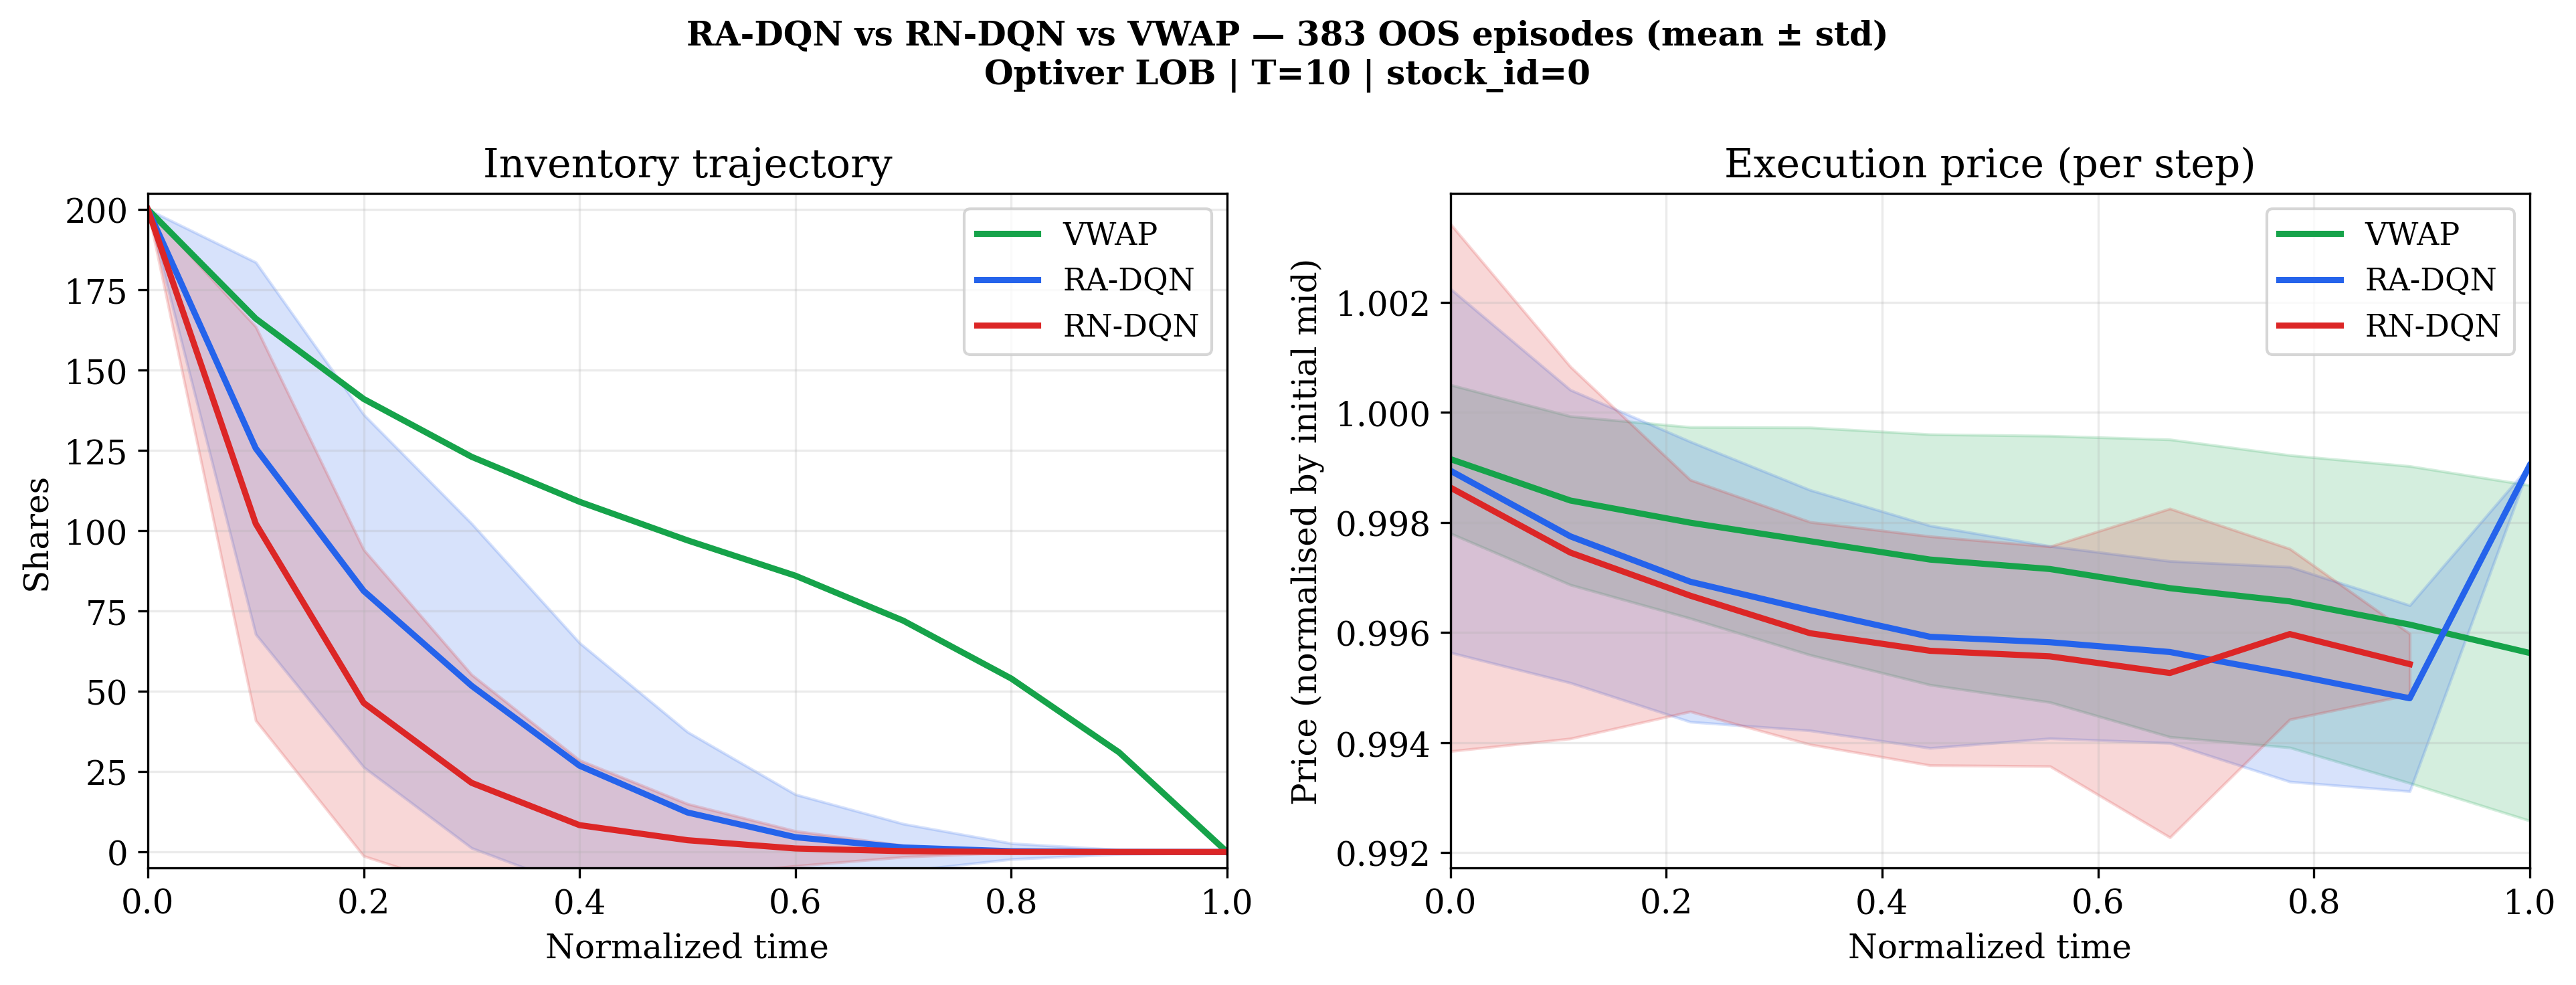
\includegraphics[width=0.90\textwidth]{figures/trajectories_CI.png}
  \end{center}
  \vspace{-6pt}
  \small
  \textbf{Left:} RA-DQN (\textcolor{myblue}{blue}) executes aggressively early;
  RN-DQN (\textcolor{myred}{red}) is more uniform;
  VWAP (\textcolor{mygreen}{green}) follows fixed U-curve.
  \textbf{Right:} RA-DQN achieves slightly better per-step prices early in the episode.
\end{frame}

\begin{frame}{Out-of-Sample Results — 112 Stocks, 42,890 Episodes}
  \begin{center}
  \renewcommand{\arraystretch}{1.5}
  \begin{tabular}{lrrrr}
    \toprule
    \textbf{Metric}
      & \textcolor{myblue}{\textbf{RA-DQN}}
      & \textcolor{myred}{\textbf{RN-DQN}}
      & \textcolor{mygreen}{\textbf{VWAP}}
      & \textcolor{mypurple}{\textbf{TWAP}} \\
    \midrule
    Mean cost (bps)
      & $23.52_{\pm0.35}$ & $\mathbf{20.20}_{\pm0.14}$ & $23.44_{\pm0.11}$ & $23.34_{\pm0.11}$ \\
    Std (bps)
      & 73.1  & 28.5  & 22.4  & 23.8  \\
    \textbf{CVaR$_{95}$ (bps)}
      & 127.7 & \textbf{56.8} & 56.6  & 57.8  \\
    \midrule
    Beats VWAP & \textbf{81\%} & \textbf{81\%} & — & — \\
    \bottomrule
  \end{tabular}\\[4pt]
  \scriptsize $\pm$SE $= \sigma/\sqrt{N}$,\; $N{=}42{,}890$
  \end{center}

  \begin{columns}[T]
    \begin{column}{0.48\textwidth}
      \begin{block}{RA vs RN — the Shen effect}
        $$\Delta\text{CVaR}_{95} = 56.8 - 127.7 = \mathbf{-70.9}\text{ bps}$$
        Shen (2014) reports $-10$ to $-15$ bps.\\
        We observe stronger effect — consistent direction.
      \end{block}
    \end{column}
    \begin{column}{0.48\textwidth}
      \begin{block}{RN-DQN vs VWAP}
        Mean cost: $\mathbf{20.2}$ vs $23.4$ bps ($-14\%$).\\
        Adaptive RL beats static U-curve in \textbf{81\%} of episodes.
      \end{block}
    \end{column}
  \end{columns}
\end{frame}

%% ============================================================
\section{Conclusion}
%% ============================================================

\begin{frame}{Summary \& Future Work}
  \begin{columns}[T]
    \begin{column}{0.50\textwidth}
      \textbf{Results:}
      \begin{itemize}
            \item[\checkmark] VWAP + RL + Risk unified
            \item[\checkmark] Risk-sensitive RL insufficient
            \item[\checkmark] CVaR-RL is next step
            \item[\checkmark] Shen (2014) replicated with GPU DQN on 112 stocks
             \item[\checkmark] RA vs RN: $\mathbf{-71}$~\textbf{bps CVaR$_{95}$}
            \item[\checkmark] Both DQN agents beat VWAP in \textbf{81\%} of episodes
            \item[\checkmark] Continuous state outperforms 23-dim one-hot
             \item[\checkmark] Parallel RA+RN training on single GPU
      \end{itemize}

      \bigskip
      \textbf{Key limitation:}\\
      CVaR is \textbf{evaluation metric}, not training objective.
    \end{column}
    \begin{column}{0.46\textwidth}
      \textbf{Future work:}
      \begin{enumerate}
        \item \textbf{CVaR in objective}\\
          \small QR-DQN / IQN: optimise tail directly
        \normalsize\item \textbf{Multiple seeds}\\
          \small Mean $\pm$ CI over 5+ runs
        \normalsize\item \textbf{Actor-Critic (PPO)}\\
          \small Continuous actions, entropy regularisation
        \normalsize\item \textbf{Richer state}\\
          \small Implied vol, realised vol, multi-level imbalance
      \end{enumerate}

      \bigskip
      \begin{alertblock}{Main takeaway}
        Risk-averse RL reduces tail execution cost
        by \textbf{71 bps CVaR$_{95}$} vs risk-neutral RL —
        correct tradeoff for CVaR-constrained institutions.
      \end{alertblock}
    \end{column}
  \end{columns}
\end{frame}

% ---- REFERENCES --------------------------------------------
\begin{frame}{References}
  \footnotesize
  \begin{enumerate}
    \item \textbf{Almgren \& Chriss (1998).}
      Optimal liquidation. \textit{Journal of Risk} 3(2), 5--39.
    \item \textbf{Nevmyvaka, Feng \& Kearns (2006).}
      RL for optimized trade execution. \textit{ICML 2006}.
    \item \textbf{Shen, Tobia, Sommer \& Obermayer (2014).}
      Risk-sensitive reinforcement learning.
      \textit{Neural Computation} 26(7), 1298--1328.
    \item \textbf{Hambly, Xu \& Yang (2021).}
      Recent advances in RL in finance. \textit{arXiv:2112.04553}.
    \item \textbf{Optiver Realized Volatility Prediction.}
      Kaggle dataset, 2021.
  \end{enumerate}
\end{frame}

% ---- THANK YOU ---------------------------------------------
\begin{frame}[plain]
  \centering
  \vspace{0.8cm}
  {\Huge\color{myblue}\textbf{Thank you!}}\\[10pt]
  {\large Questions?}\\[20pt]

  \begin{columns}[c]
    \begin{column}{0.28\textwidth}
      \centering
      \qrcode[height=3cm]{https://github.com/matvei-lukianov/AMS_517_optimal_execution}
    \end{column}
    \begin{column}{0.68\textwidth}
      \footnotesize
      \textbf{Code \& Results:}\\[4pt]
      \texttt{github.com/matvei-lukianov/}\\
      \texttt{AMS\_517\_optimal\_execution}\\[10pt]
      Reproducible on NVIDIA RTX 3080\\
      in $\approx$30 min with Optiver data.
    \end{column}
  \end{columns}
\end{frame}

\end{document}